% LaTeX Template for Project Report, Version 2.0
% (Abstracted from a Major Project Report at CSED, NIT Calicut but can be
% modified easily to use for other reports also.)
%
% Released under Creative Commons Attribution license (CC-BY)
% Info: http://creativecommons.org/licenses/by/3.0/
%
% Created by: Kartik Singhal
% BTech CSE Batch of 2009-13
% NIT Calicut
% Contact Info: kartiksinghal@gmail.com
%
% It is advisable to learn the basics of LaTeX before using this template.
% A good resource to start with is http://en.wikibooks.org/wiki/LaTeX/
%
% All template fields are marked with a pair of angular brackets e.g. <title here>
% except for the ones defining citation names in ref.tex.
%
% Empty space after chapter/section/subsection titles can be used to insert text.
%
% Just compile this file using pdflatex after making all required changes.

\documentclass[12pt,a4paper]{report}
\usepackage[pdftex]{graphicx} %for embedding images
\usepackage{url} %for proper url entries
\usepackage[bookmarks, colorlinks=false, pdfborder={0 0 0}, pdftitle={RakthaDatha}, pdfauthor={B130153CS , B130253CS}, pdfsubject={Web programming}, pdfkeywords={"WEBP"}]{hyperref} %for creating links in the pdf version and other additional pdf attributes, no effect on the printed document
%\usepackage[final]{pdfpages} %for embedding another pdf, remove if not required

\begin{document}
%\renewcommand\bibname{References} %Renames "Bibliography" to "References" on ref page

%include other pages
\begin{titlepage}

\begin{center}

\textup{\small {\bf CS4042 Project} \\ Report}\\[0.2in]

% Title
\Large \textbf {Raktha Datha}\\[0.5in]

%       \small \emph{Submitted in partial fulfillment of\\
%        the requirements for the award of the degree of}
%        \vspace{.2in}

%       {\bf Bachelor of Technology \\in\\ Computer Science and Engineering}\\[0.5in]

% Submitted by
\normalsize Submitted by \\
\begin{table}[h]
\centering
\begin{tabular}{lr}\hline \\
Roll No & Names of Students \\ \\ \hline
\\
B130153CS & SANATH DAVIS \\
B130253CS & SHRIMADHAV U K \\ \\ \hline
%B130461CS & SIMSARUL HAQ V \\ \\ \hline
\end{tabular}
\end{table}

\vspace{.1in}
Under the guidance of\\
{\textbf{Mr. Sreenivasan M}}\\
{\textbf{Ms. Sreekala S}}\\[0.2in]

\vfill

% Bottom of the page

\includegraphics[width=0.18\textwidth]{./nitc-logo}\\[0.1in]
\Large{Department of Computer Science and Engineering}\\
\normalsize
\textsc{National Institute of Technology Calicut}\\
Calicut, Kerala, India -- 673 601 \\
\vspace{0.2cm}
Monsoon Semester 2015

\end{center}

\end{titlepage}

%\newpage
\thispagestyle{empty}

\begin{center}

\huge{Department of Computer Science and Engineering}\\[0.5cm]
\normalsize
\textsc{National Institute of Technology Calicut}\\[2.0cm]

\emph{\LARGE Certificate}\\[2.5cm]
\end{center}
\normalsize This is to certify that this is a bonafide record of the project presented by the students whose names are given below during <Monsoon/Winter and Year here> in partial fulfilment of the requirements of the degree of Bachelor of Technology in Computer Science and Engineering.\\[1.0cm]

\begin{table}[h]
\centering
\begin{tabular}{lr}
Roll No & Names of Students \\ \\ \hline
\\
<Roll no here> & <Name here> \\ 
<Roll no here> & <Name here> \\
<Roll no here> & <Name here> \\
\end{tabular}
\end{table}

\vfill


% Bottom of the page
\begin{flushright}
<Guide name here>\\
(Project Guide)\\[1.5cm]
<Coordinator name here>\\
(Course Coordinator)\\
\end{flushright}

\begin{flushleft}
Date:
\end{flushleft}

%\vspace{2in}
\begin{abstract}

This report describes our group's implementation of a blood donation
management system. We used the Entity-Relationship model to design
a database that will store and organize the library's data. We have
created the database using SQL and populated it with some sample
data. The system can keep track of blood donor informations, patients who have donated blood,
and the relationships
between them. Using MySQL, and PHP, we have
created an Internet-based graphical user interface that allows
the patients and the donors to access the system remotely.

\end{abstract}


\pagenumbering{roman} %numbering before main content starts
%\tableofcontents
%\listoffigures

\newpage
\pagenumbering{arabic} %reset numbering to normal for the main content

%\chapter{Problem Definition}
\section{Problem Description}
%\subsection{<Sub-section title>}
%<Problem Definition here>

\vspace{5mm} %5mm vertical space

The Raktha Datha (blood donation management) system aims to create an e-Information about the blood donors and organizations
that are related to donating the blood.
Through this application any person who is interested in donating blood can register themself on the website.
If any organization wants to register itself with this site they can also register.
Moreover if any general consumer wants a particular blood group he can request online by taking help of this website.
Admin is the main authority who can do addition, deletion, and modification if required.

%\vspace{5mm} %5mm vertical space
%The standards of security and data protective mechanism have been given a big choice for proper usage.
%The application takes care of different modules and their associated reports,
%which are produced as per the applicable strategies and standards that are put forwarded by the administrative staff.
 %objective changed to problem definition
%\chapter{Introduction}

%\section{Background and Recent Research}
%\subsection{<any sub section here>}

%\subsection{Literature Survey}

%\subsubsection{<Sub-subsection title>}
%some text\cite{citation-1-name-here}, some more text

%\subsubsection{<Sub-subsection title>}
%even more text\footnote{<footnote here>}, and even more.

\section{Motivation}

This report will provide a detailed account of the processes our group
used to design and implement a database that can be used to manage
a blood donation system. Each subsection of the report will correspond to an
important feature of database design.

\section{Database Schema}

\subsection{BDC Employee}

\begin{tabular}{ | c | c | c | c | c | c | c | }
 \hline
 EMP ID & BDC ID & F NAME & L NAME & DESIGNATION & DATE OF JOIN & PASSWORD \\
 \hline
\end{tabular}

\subsection{BDC Employee}

\begin{tabular}{ | c | c | c | c | c | c | c | }
 \hline
 EMP ID & BDC ID & F NAME & L NAME & DESIGNATION & DATE OF JOIN & PASSWORD \\
 \hline
\end{tabular}

\subsection{BDC Employee}

\begin{tabular}{ | c | c | c | c | c | c | c | }
 \hline
 EMP ID & BDC ID & F NAME & L NAME & DESIGNATION & DATE OF JOIN & PASSWORD \\
 \hline
\end{tabular}

\subsection{BDC Employee}

\begin{tabular}{ | c | c | c | c | c | c | c | }
 \hline
 EMP ID & BDC ID & F NAME & L NAME & DESIGNATION & DATE OF JOIN & PASSWORD \\
 \hline
\end{tabular}

\subsection{BDC Employee}

\begin{tabular}{ | c | c | c | c | c | c | c | }
 \hline
 EMP ID & BDC ID & F NAME & L NAME & DESIGNATION & DATE OF JOIN & PASSWORD \\
 \hline
\end{tabular}

\subsection{BDC Employee}

\begin{tabular}{ | c | c | c | c | c | c | c | }
 \hline
 EMP ID & BDC ID & F NAME & L NAME & DESIGNATION & DATE OF JOIN & PASSWORD \\
 \hline
\end{tabular}

\subsection{BDC Employee}

\begin{tabular}{ | c | c | c | c | c | c | c | }
 \hline
 EMP ID & BDC ID & F NAME & L NAME & DESIGNATION & DATE OF JOIN & PASSWORD \\
 \hline
\end{tabular}

\subsection{BDC Employee}

\begin{tabular}{ | c | c | c | c | c | c | c | }
 \hline
 EMP ID & BDC ID & F NAME & L NAME & DESIGNATION & DATE OF JOIN & PASSWORD \\
 \hline
\end{tabular}


\section{Entity Relationship Diagram}
\begin{figure}[htb]
\centering
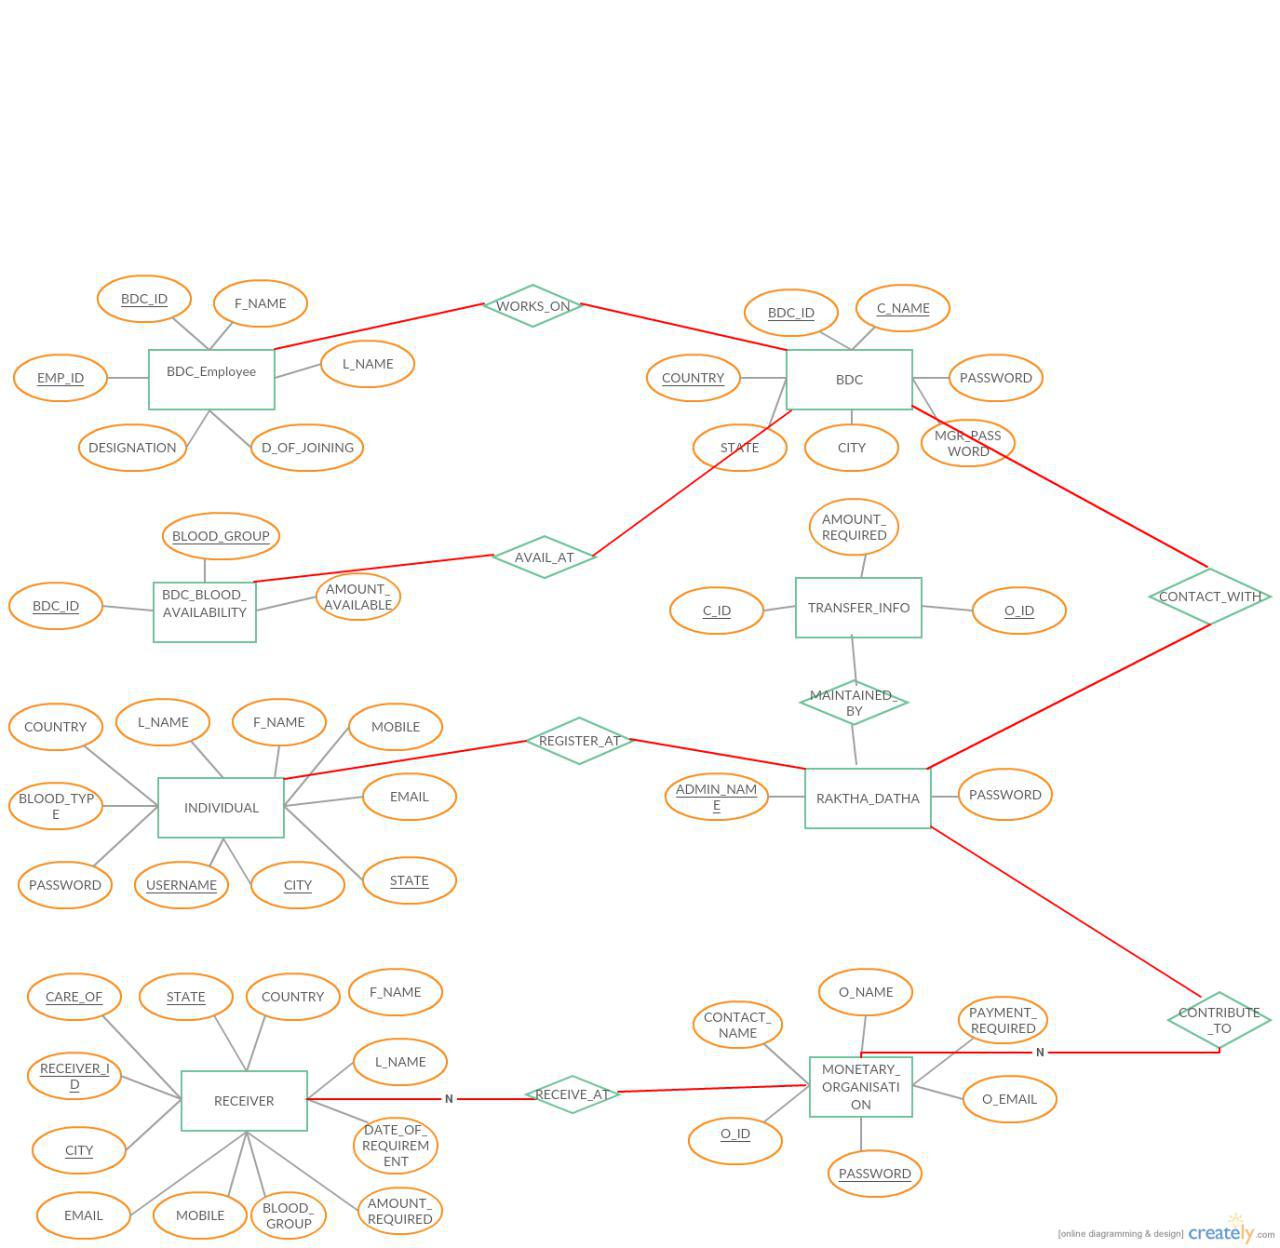
\includegraphics[scale=0.3]{./er} % e.g. insert ./image for image.png in the working directory, adjust scale as necessary
%\caption{<Caption here>}
\label{fig:label} % insert suitable label, this is used to refer to a fig from within the text as shown above
\end{figure}

\section{Glossary}
BDC Employee : Blood Donation Centre Employee
 %literature survey included in this
%\chapter{Work Done}

\section{<Section title>}

\subsection{<Sub-section title>}

\subsection{<Sub-section title>}
some text\cite{citation-2-name-here}, some more text
\subsection{<Sub-section title>}

\subsection{<Sub-section title>}

Refer figure \ref{fig:label}.

\begin{figure}[htb]
\centering

\includegraphics[scale=0.3]{./glider} % e.g. insert ./image for image.png in the working directory, adjust scale as necessary
\caption{<Caption here>}
\label{fig:label} % insert suitable label, this is used to refer to a fig from within the text as shown above
\end{figure}

\subsection{<Sub-section title>}


\section{<Section title>}


%\chapter{Future Work}

<Future work here>

%\chapter{Conclusion}

<Conclusion here>

%\cleardoublepage
%\pagebreak
\phantomsection
\addcontentsline{toc}{chapter}{Acknowledgements}
\chapter*{Acknowledgments}
\vspace{1.0in}
<Acknowledgements here>
\\
\\
\\ 
\\
<Name here> \\ 
\\
<Month and Year here>\\
{National Institute of Technology Calicut}\\
\newpage

%\cleardoublepage
%\pagebreak
\phantomsection
\addcontentsline{toc}{chapter}{References}
\begin{thebibliography}{99}

\bibitem{citation-1-name-here}<Name of the reference here>,\ \url{<url here>}

\bibitem{citation-2-name-here}<Name of the reference here>,\ \url{<url here>}

\end{thebibliography}


\end{document}
